\begin{frame}
  \frametitle{Introducción: ¿Qué es el Mercurio?}
  \begin{itemize}
    \item \textbf{Símbolo químico:} \ce{Hg}
    \item \textbf{Número atómico:} 80
    \item Conocido comúnmente como azogue.
    \item Es el único elemento metálico que es líquido a temperatura y
      presión estándar.
    \item Esta singularidad le confiere un conjunto de propiedades
      fascinantes que lo distinguen de todos los demás metales.
  \end{itemize}
\end{frame}


\begin{frame}
  \frametitle{La Esencia del Mercurio: Composición Atómica}
  \begin{itemize}
    \item \textbf{Número Atómico (Z): 80}
      \begin{itemize}
        \item Cada átomo posee 80 protones en su núcleo.
      \end{itemize}
      \medskip
    \item \textbf{Masa Atómica:}
      \begin{itemize}
        \item Aproximadamente 200.59 u.
      \end{itemize}
      \medskip
    \item \textbf{Configuración Electrónica: \ce{[Xe] 4f^{14} 5d^{10} 6s^{2}}}
      \begin{itemize}
        \item Sus capas de electrones llenas y estables explican su
          bajo punto de fusión.
      \end{itemize}
      \medskip
    \item \textbf{Isótopos Estables:}
      \begin{itemize}
        \item Tiene 7 isótopos naturales, siendo el \ce{^{202}Hg} el
          más abundante.
      \end{itemize}
  \end{itemize}
\end{frame}


\begin{frame}
  \frametitle{Características Físicas}
  \begin{columns}[T]
    \begin{column}{0.5\textwidth}
      \begin{itemize}
        \item \textbf{Estado:} Líquido a temperatura ambiente.
          \begin{itemize}
            \item \textbf{Punto de Fusión:} $-38.83 \,^{\circ}\text{C}$
            \item \textbf{Punto de Ebullición:} $356.73 \,^{\circ}\text{C}$
          \end{itemize}
          \medskip
        \item \textbf{Apariencia:}
          \begin{itemize}
            \item Líquido denso y pesado.
            \item Color blanco plateado, muy brillante.
          \end{itemize}
          \medskip
        \item \textbf{Densidad:}
          \begin{itemize}
            \item \textbf{13.534 g/cm$^3$}
          \end{itemize}
      \end{itemize}
    \end{column}
    \begin{column}{0.5\textwidth}
      \begin{figure}
        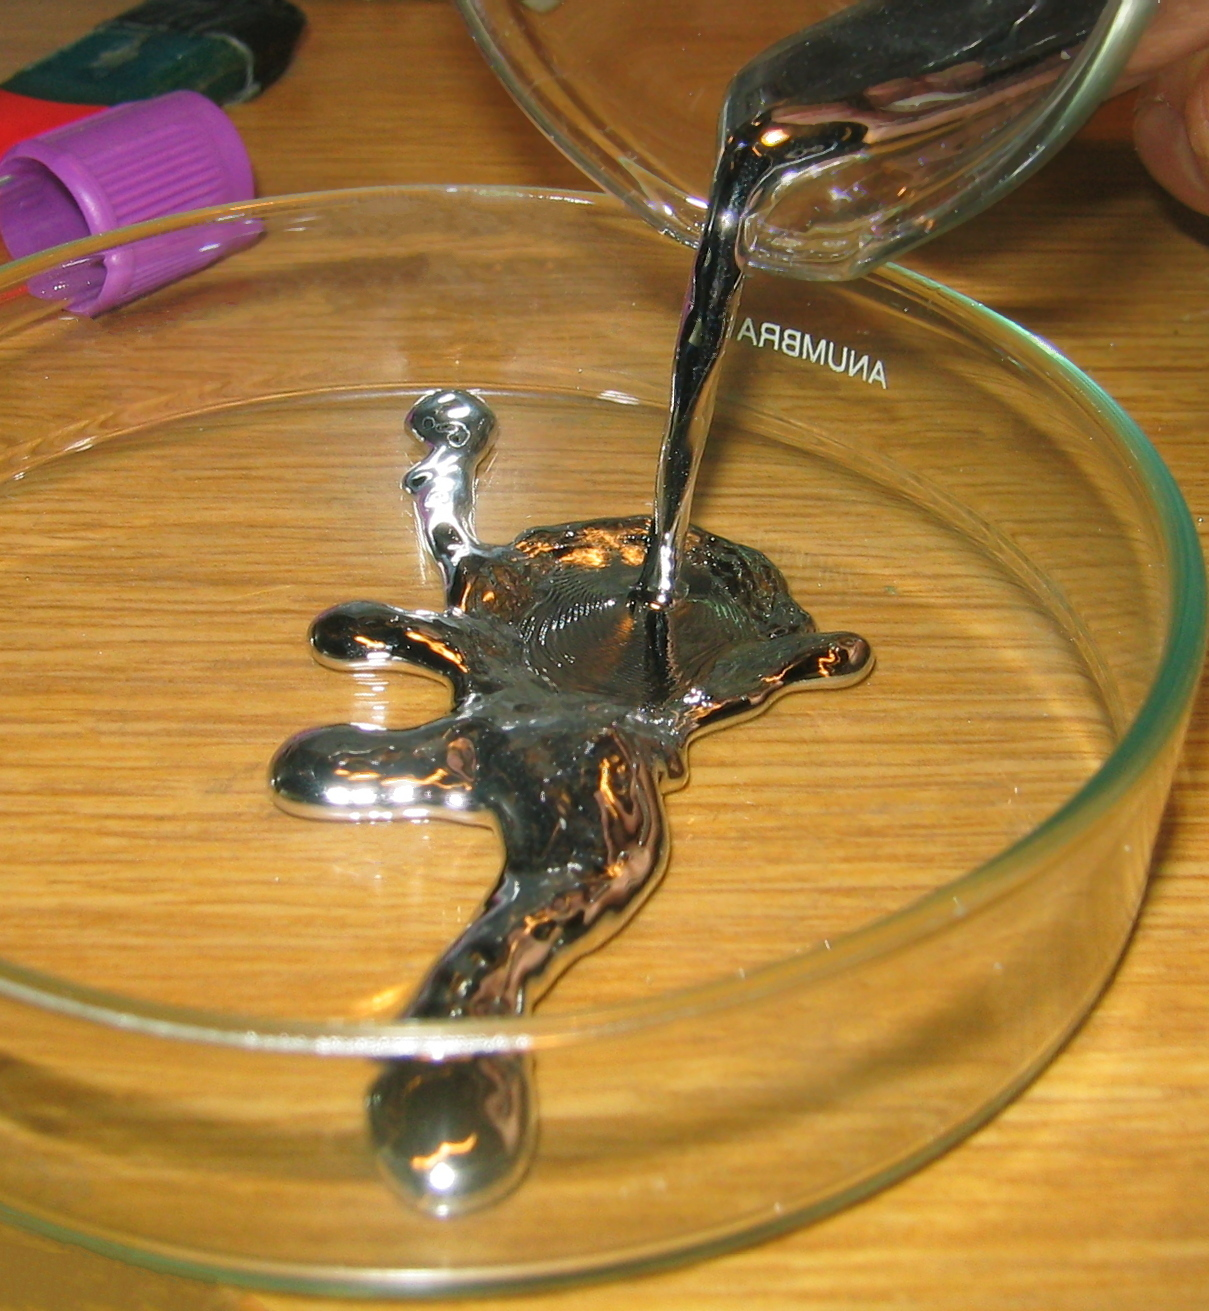
\includegraphics[width=0.7\textwidth]{../figures/liquidmercury.jpg}
        \caption{Mercurio líquido.}
      \end{figure}
    \end{column}
  \end{columns}
\end{frame}


\begin{frame}
  \begin{itemize}
    \item \textbf{Conductividad:}
      \begin{itemize}
        \item Es un mal conductor del calor.
        \item Pero un buen conductor de la electricidad.
      \end{itemize}
      \medskip
    \item \textbf{Tensión Superficial:}
      \begin{itemize}
        \item Posee una tensión superficial muy alta, lo que
          hace que forme gotas perfectamente redondeadas.
      \end{itemize}
      \medskip
    \item \textbf{Volatilidad:}
      \begin{itemize}
        \item Se evapora lentamente a temperatura ambiente.
        \item Forma vapores inodoros e incoloros que son tóxicos.
      \end{itemize}
  \end{itemize}
\end{frame}


\begin{frame}
  \frametitle{Comportamiento Químico}
  \begin{columns}[T]
    \begin{column}{0.5\textwidth}
      \begin{itemize}
        \item \textbf{Reactividad con el Aire:}
          \begin{itemize}
            \item No reacciona con el oxígeno a temperatura
              ambiente. Se oxida lentamente si se calienta para
              formar óxido de mercurio (\ce{HgO}).
          \end{itemize}
          \medskip
        \item \textbf{Reacción con Ácidos:}
          \begin{itemize}
            \item No reacciona con la mayoría de los ácidos diluidos.
            \item Sí reacciona con ácidos oxidantes fuertes.
          \end{itemize}
          \medskip
        \item \textbf{Estados de Oxidación:}
          \begin{itemize}
            \item Sus estados más comunes son +1 (mercuroso) y
              +2 (mercúrico).
          \end{itemize}
      \end{itemize}
    \end{column}
    \begin{column}{0.5\textwidth}
      \begin{figure}
        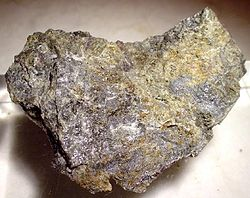
\includegraphics[width=0.7\textwidth]{../figures/solidmercury.jpg}
        \caption{Muestra del mineral Cinabrio (\ce{HgS}).}
      \end{figure}
    \end{column}
  \end{columns}
\end{frame}


\begin{frame}
  \begin{itemize}
    \item \textbf{Formación de Amalgamas:}
      \begin{itemize}
        \item Tiene la capacidad única de disolver muchos otros metales
          (oro, plata, estaño) para formar aleaciones llamadas amalgamas.
        \item No forma amalgama con el hierro.
      \end{itemize}
      \medskip
    \item \textbf{Reacción con Azufre:}
      \begin{itemize}
        \item Reacciona fácilmente con el azufre.
        \item Esta reacción es útil para controlar derrames, ya que el
          compuesto resultante (\ce{HgS}) es mucho menos peligroso.
      \end{itemize}
  \end{itemize}
\end{frame}
